\label{impl:overview}
This section will give an overview of the different components and the overall flow of \pyt{}.
An illustration giving an abstract overview can be seen on \cref{figure:implementation_overview}.

\begin{figure}
  \begin{tikzpicture}
\newcommand\XLabel{7}
\newcommand\XNode{10}
\newcommand\XEngines{14}
\newcommand\TextWidth{3}
\tikzset{>=latex}

%\draw[help lines] (5,5) grid (15,20);

%%%%%%%%%%%% MID STRUCTURE %%%%%%%%%%%%%%%%%%%
\node[inner sep=10pt] (code) at (\XNode,18)
    {
\includegraphics[width=.1\textwidth]{./figures/dot_files/implementation_overview_images/source_code.png}};
\node[text width=\TextWidth{}cm] at (\XLabel,18) {\hfill{}Source code};

\node[inner sep=10pt] (ast) at (\XNode,15)
    {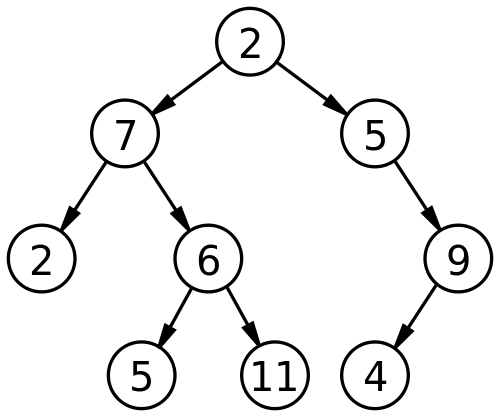
\includegraphics[width=.15\textwidth]{./figures/dot_files/implementation_overview_images/ast.png}};
\node[text width=\TextWidth{}cm] at (\XLabel,15) {\hfill{}AST};

\node[inner sep=10pt] (cfg) at (\XNode,11)
    {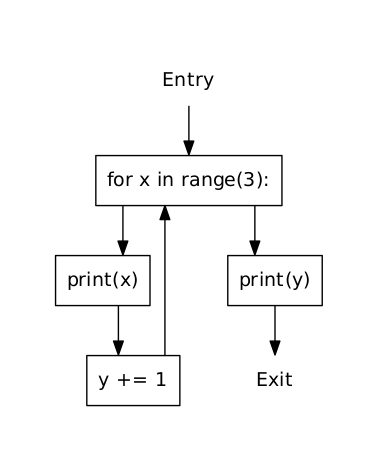
\includegraphics[width=.2\textwidth]{./figures/dot_files/implementation_overview_images/for_complete.png}};
\node[text width=\TextWidth{}cm] at (\XLabel,11) {\hfill{}CFG};

\node[inner sep=10pt] (engine) at (\XNode,7)
    {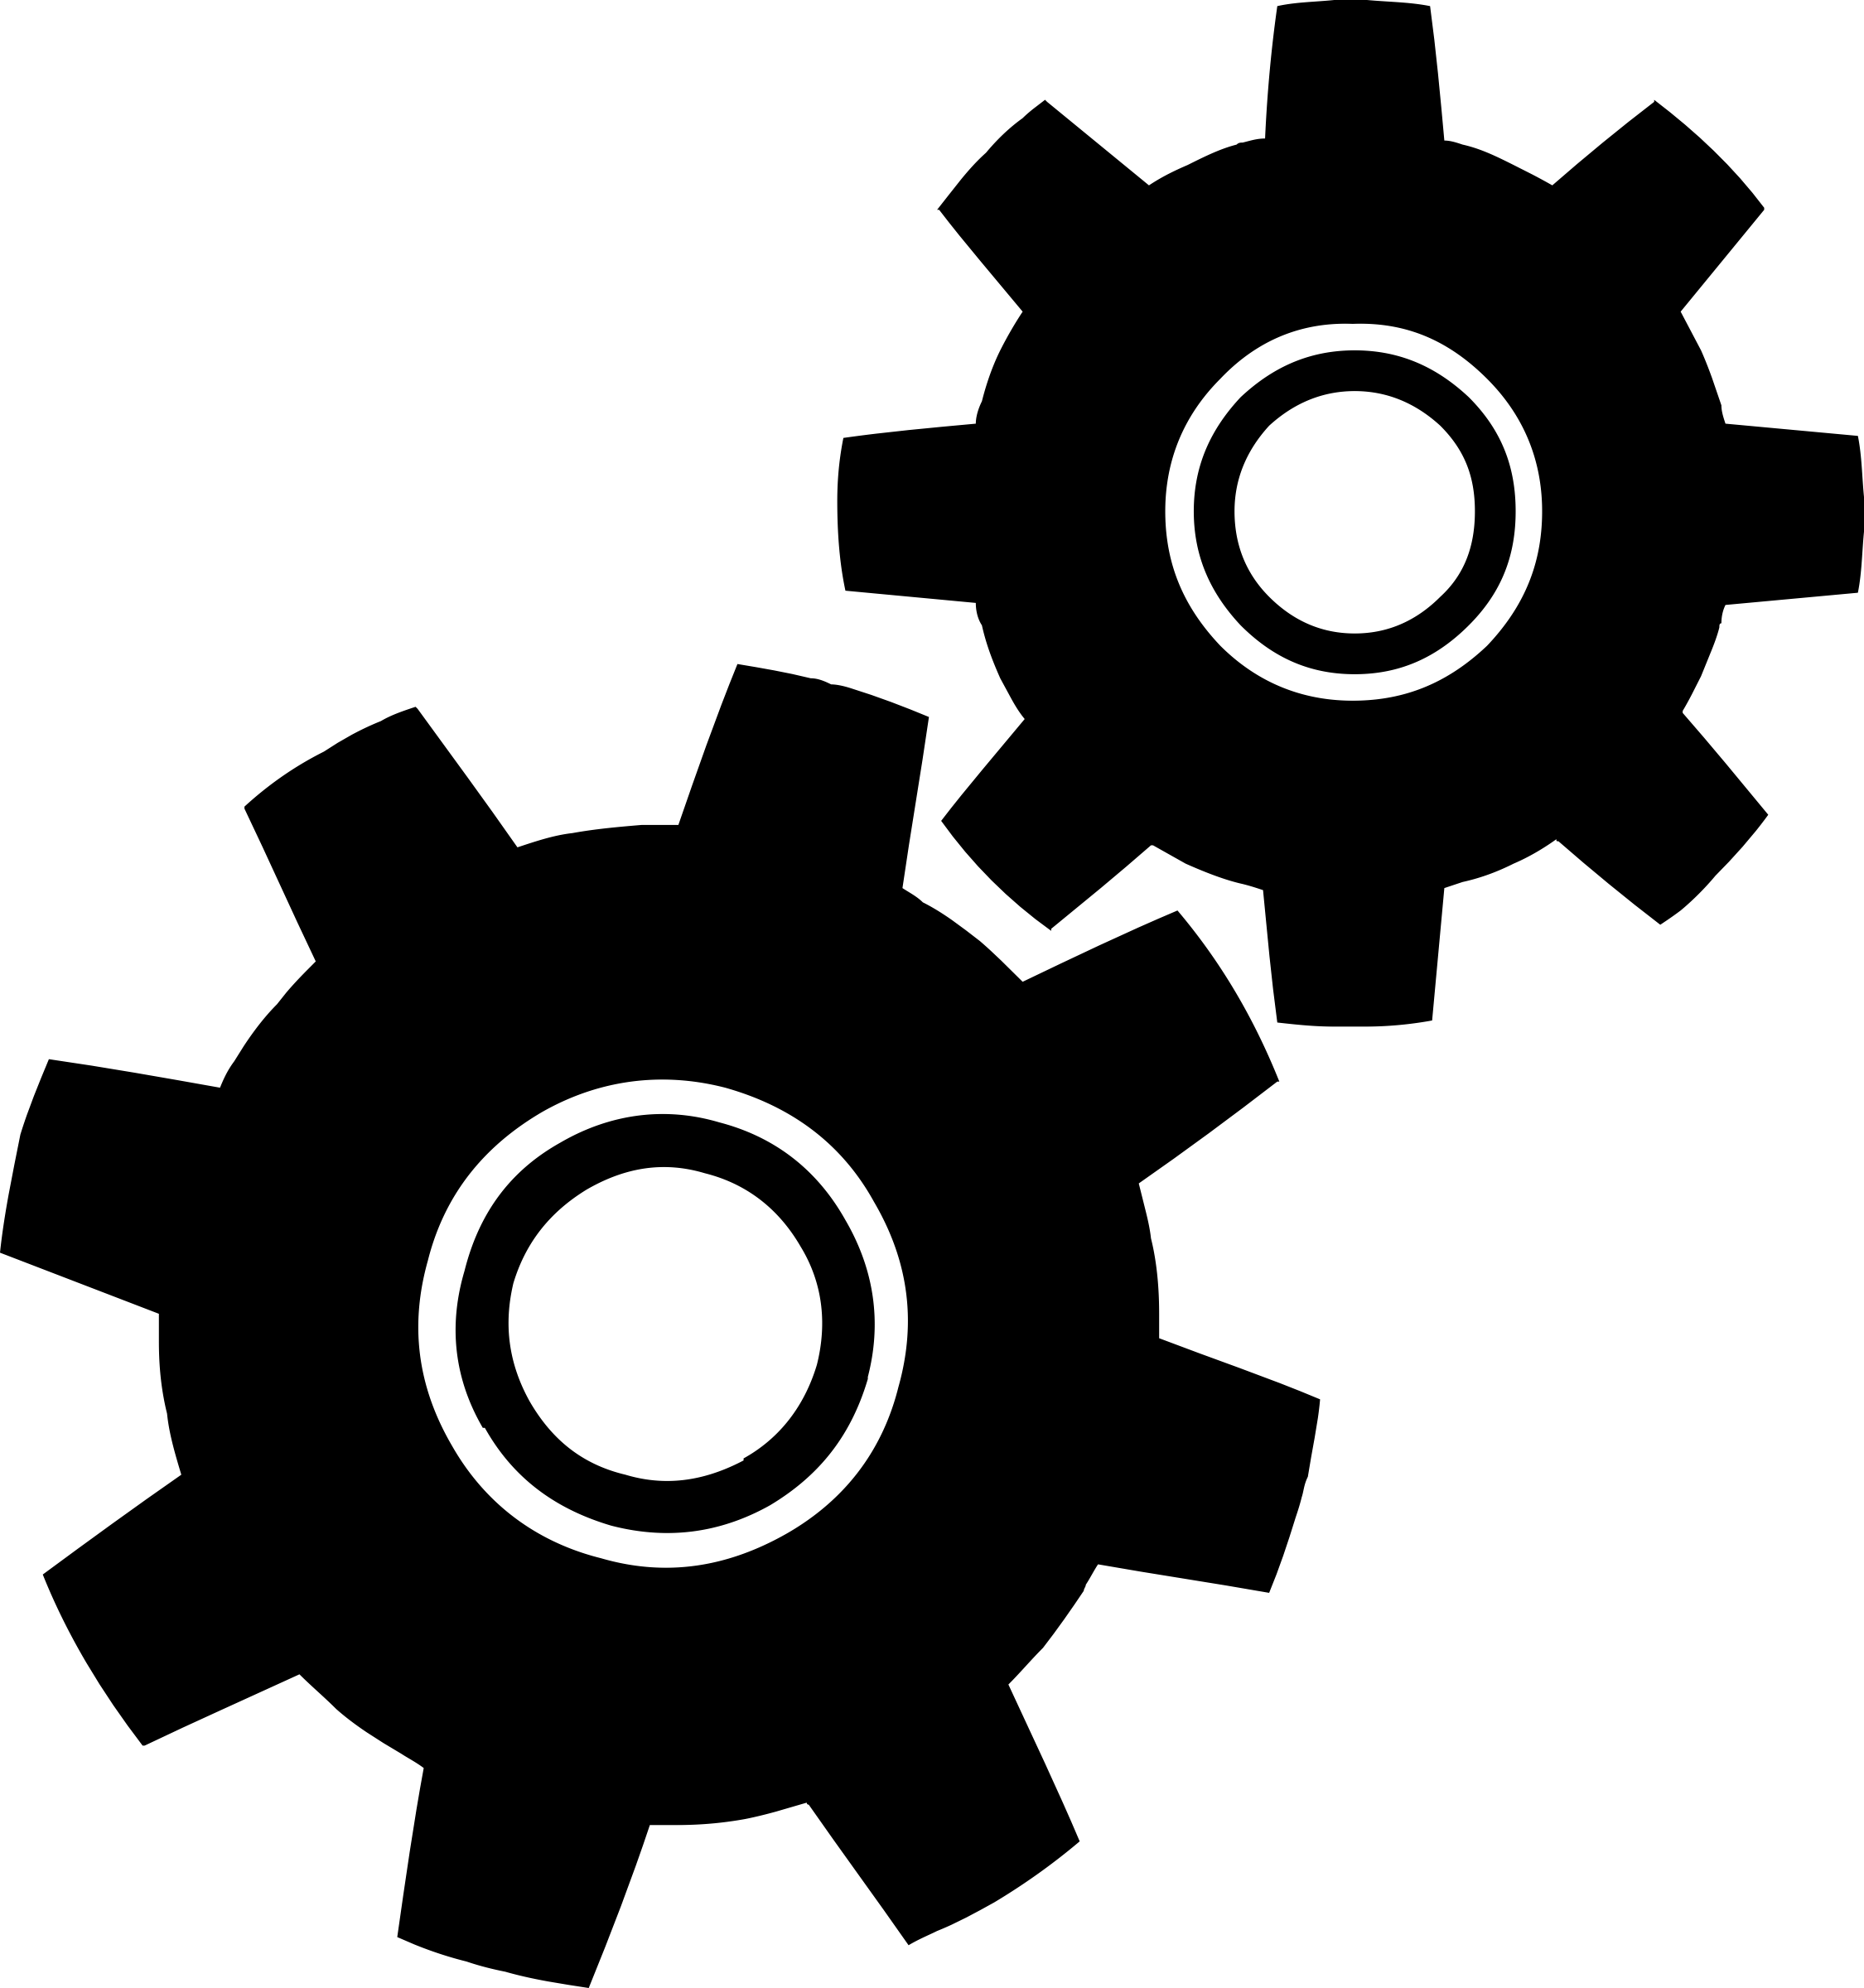
\includegraphics[width=.1\textwidth]{./figures/dot_files/implementation_overview_images/cog_wheel.png}};
\node[text width=\TextWidth{}cm] at (\XLabel,7) {\hfill{}Engine};

\node[inner sep=10pt] (algorithm) at (\XNode,4)
    {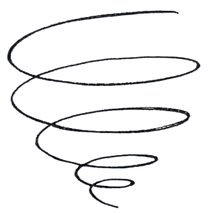
\includegraphics[width=.1\textwidth]{./figures/dot_files/implementation_overview_images/spiral.png}};
\node[text width=\TextWidth{}cm] at (\XLabel,4) {\hfill{}Fixed Point \\ \hfill{}Algorithm};

\node[inner sep=10pt] (vulnerabilities) at (\XNode,1)
    {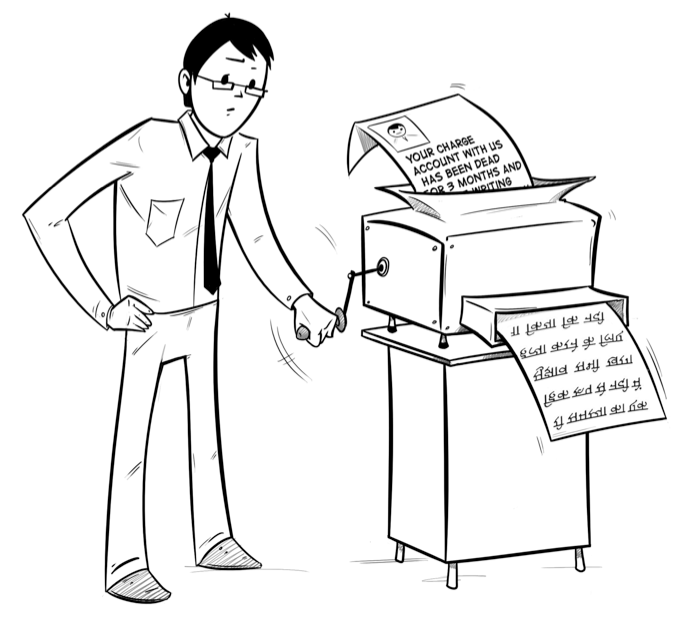
\includegraphics[width=.15\textwidth]{./figures/dot_files/implementation_overview_images/vulnerability.png}};
\node[text width=\TextWidth{}cm] at (\XLabel,1) {\hfill{}Vulnerabilities};

%%%%%%%%%%%%%%%%%%%% ENGINES %%%%%%%%%%%%%%%%%%%%%%%%
\node[inner sep=10pt] (flask) at (\XEngines,11)
    {
\includegraphics[width=.2\textwidth]{./figures/dot_files/implementation_overview_images/flask_text.png}};

\node[inner sep=5pt] (django) at (\XEngines,9)
    {
\includegraphics[width=.13\textwidth]{./figures/dot_files/implementation_overview_images/django.png}};

\node[label=below:{Other}, inner sep=5pt] (other_engine) at (\XEngines,7)
    {
\includegraphics[width=.05\textwidth]{./figures/dot_files/implementation_overview_images/question_mark.png}};

%%%%%%%%%%%%%%%% ANALYSIS %%%%%%%%%%%%%%%%%%%%%%%%%    
\node[label=below:{Analysis}, inner sep=10pt] (analysis) at (\XEngines,4)
    {
\includegraphics[width=.1\textwidth]{./figures/dot_files/implementation_overview_images/analysis.png}};

\node[text width=2cm, inner sep=10pt] (reaching) at (18,7) {Reaching Definitions};
\node[text width=2cm, inner sep=10pt] (liveness) at (18,4) {Liveness};

\node[label=below:{Other}, inner sep=5pt] (other_analysis) at (18,1)
    {
\includegraphics[width=.05\textwidth]{./figures/dot_files/implementation_overview_images/question_mark.png}};


\draw[->] (code) -- (ast);
\draw[->] (ast) -- (cfg);
\draw[->] (cfg) -- (engine);
\draw[->] (engine) -- (algorithm);
\draw[->] (algorithm) -- (vulnerabilities);

\draw[->] (flask) -- (engine);
\draw[->] (django) -- (engine);
\draw[->] (other_engine) -- (engine);

\draw[<->] (algorithm) -- (analysis);
\draw[->] (reaching) -- (analysis);
\draw[->] (liveness) -- (analysis);
\draw[->] (other_analysis) -- (analysis);

\end{tikzpicture}
  \caption{An abstract overview of the implementation of \pyt{}, showing the main components and the flow}
  \label{figure:implementation_overview}
\end{figure}

The illustration shows how  \pyt{} takes the source code as input, manipulates it and finally outputs a list of potential vulnerabilities.
The process will be described in the following on a general level.

\begin{itemize}
\item The source code is parsed to an abstract syntax tree (denoted as AST) representation of each file in the project being analysed.
The AST is generated using the standard Python library \texttt{ast}\cite{python_ast}.
\item The AST is systematically traversed and turned into a control flow graph by the CFG component.
\item The resulting CFG is not prepared for the analysis by a framework adaptor, depending on the web framework used in the source code.
  The default adaptor is the Flask adaptor, but a similar module for Django applications could be devised.
\item The fixed point algorithm is applied on the CFG and the resulting constraints are annotated on each CFG node
  The fixed point module is flexible which means that the analysis can be substituted or extended with other analyses.
  By default \pyt{} uses the extended reaching definitions analysis presented in the previous chapter.
\item At last the annotated CFG is investigated, and a log is provided to the user giving precise information about the potential vulnerabilities found by the analysis
\end{itemize}
